\section{Integration of the Subsystems} \label{sec:integration}

% ===== Measure of success for the complete system ===== %
After the tests are conducted for subsystems and the optimal solutions are determined, the subsystems will be integrated. 

Integration plan for subsystems is scheduled as below:
\begin{itemize}
\item Integration of mechanical parts.
\item Integration of exterior design with electronic equipments.
\item Integration of camera and microprocessor.
\item Algorithm related integration on microprocessor.
\item Integration of microprocessor and mechanical part.
\end{itemize}

Being satisfied the subsystem requirements, integration between the subsystems will be done. The integration procedure can be seen below:
\begin{itemize}
    \item Integration of the box with the camera and microprocessor unit.
    \item Integration of the dog deterring systems with the box.
    \item Integration of the exterior design with the food mechanism.
    \item Integration of the box with the computer vision submodule.
\end{itemize}

Measure of success can be seen below:
\begin{itemize}
    \item \%90 of successfully identifying cats.
    \item \%90 of successfully identifying dogs.
    \item \%70 of successfully deterring dogs from the area.
    \item Giving right amount of food to cats at \%80.
    \item At least 5 hours working system without being charged.
\end{itemize}


\begin{figure}[h!]
    \centering
    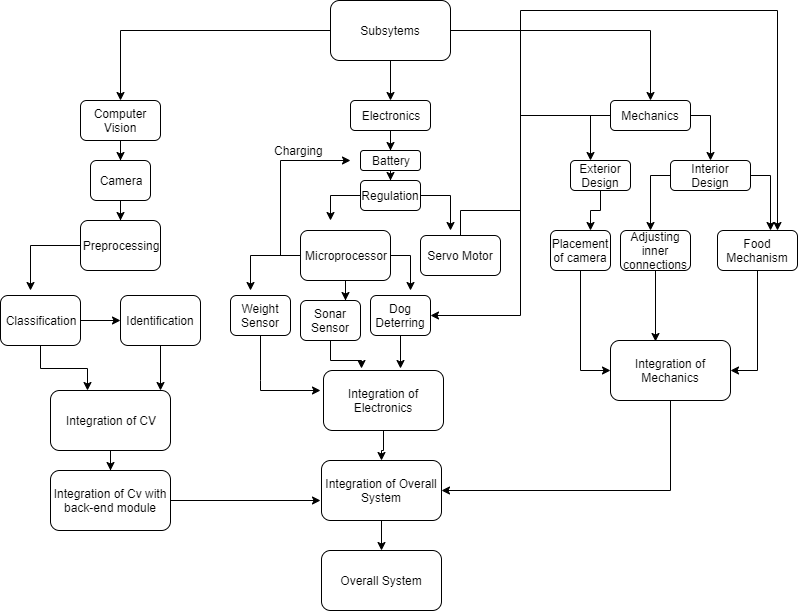
\includegraphics[width=\linewidth]{img/FlowChart.png}
    \caption{Flow Chart for Overall System}
    \label{fig:Flow Chart for Overall System}
\end{figure}


In figure \ref{fig:Flow Chart for Overall System} one can observe the subsystems and their related works, in a Flow Chart. Firstly all of the subsystems will finalize their products according to the desired specifications. The jobs for every single subsystem can be seen in above. After every subsystem finalizes their product, the integration of the subsystems will be done. Since everything is nested and parts rely on other parts to function properly, the implementation process should be approached with caution. The malfunctioning of a single block can disrupt the whole system. The main idea to avoid such a case is to write test codes for each module, write info logging to a separate file to detect where the system goes wrong. Another important aspect is to test the whole system after each module's implementation to the existing system. This way it will be easier to make sure the functioning is proper and the new arriving module doesn't cause any problems. 
